\documentclass[a4paper]{article}
\usepackage[utf8]{inputenc}
\usepackage[spanish]{babel}

\usepackage{xcolor}     % \textcolor
\usepackage{amsmath}    % 
\usepackage{caratula}   % caratula del TP
\usepackage{url}

% Figuras y graficos
\usepackage{float}
\usepackage{graphicx}
\usepackage{pgfplotstable}

% Tablas
\usepackage{xltabular}


\newcommand{\norm}[1]{\left\lVert#1\right\rVert}%
\newcommand{\pint}[1]{\left\langle#1\right\rangle}%


% ********************************************************* %
% ~~~~~~~~         Formato de las páginas         ~~~~~~~~~ %
% ********************************************************* %

\usepackage{csquotes}
\usepackage{fancyhdr}
\pagestyle{fancy}

%\renewcommand{\chaptermark}[1]{\markboth{#1}{}}
\renewcommand{\sectionmark}[1]{\markright{\thesection\ - #1}}

\fancyhf{}

\fancyhead[LO]{Sección \rightmark} % \thesection\ 
\fancyfoot[RO]{\thepage}
\renewcommand{\headrulewidth}{0.5pt}
\renewcommand{\footrulewidth}{0.5pt}
\setlength{\hoffset}{-0.8in}
\setlength{\textwidth}{16cm}
%\setlength{\hoffset}{-1.1cm}
%\setlength{\textwidth}{16cm}
\setlength{\headsep}{0.5cm}
\setlength{\textheight}{25cm}
\setlength{\voffset}{-0.7in}
\setlength{\headwidth}{\textwidth}
\setlength{\headheight}{13.1pt}
\renewcommand{\baselinestretch}{1.1}  % line spacing

%**********************************************************%


\begin{document}

\thispagestyle{empty}
\materia{Métodos Numericos}
\submateria{Primer Cuatrimestre de 2020}
\titulo{Trabajo Práctico 2}
\subtitulo{Reconocimiento de dígitos}
\integrante{Manuel Panichelli}{72/18}{panicmanu@gmail.com}
\integrante{Tomas Tropea}{115/18}{tomastropeaa@gmail.com}
\integrante{Ignacio Alonso Rehor}{195/18}{arehor.ignacio@gmail.com}

\maketitle
\newpage

\thispagestyle{empty}
\tableofcontents

% Objetivos generales
% 1 Implementar el m´etodo kNN.
% 2 Implementar el m´etodo de PCA y combinarlo con kNN.
% 3 Experimentar variando: k, α, K, Analizar los resultados en t´erminos de
% diferentes m´etricas (mirando al menos la tasa de efectividad) aplicando
% cross validation sobre la base de training.
% 4 Para encontrar los autovectores necesarios, utilizar el M´etodo de la
% Potencia + Deflaci´on.

\section{Abstract}

En este informe se aborda la problemática de reconocimiento de dígitos, con un clasificador que utilice el algoritmo de kNN \textit{(k Nearest Neighbors)} por si solo y en combinación con PCA \textit{(Principal Component Analysis)}, ambos programados por nosotros usando Eigen. Además, se consideran variaciones de kNN que apliquen pesos a los votos de los vecinos.

Se analiza el comportamiento de cada uno y se optimizan sus parámetros con \textit{Simulated Annealing}. También se observa como se comportan luego de ser optimizados bajo ciertas métricas y variaciones de parámetros. Finalmente se concluye cual es mejor y se hace un submission con el a la competencia \textit{Digit Recognizer} de Kaggle.

\textit{\textbf{keywords:} OCR; kNN; PCA; Optimización}

\section{Introducción}

El reconocimiento de dígitos ha ocupado un lugar importante en el campo de \textit{Machine Learning} en las ultimas décadas. Este ha sido una de las motivaciones para impulsar el desarrollo de nuevos algoritmos, cada vez mas complejos, dentro del área de \textit{Computer Vision}. A pesar de estar ampliamente estudiado, sigue siendo de interés para comenzar como un primer paso en el campo, o incluso para experimentar con nuevas técnicas.

A la hora de clasificar digitos, existen técnicas muy complejas pero también otras muy simples conceptualmente, que de todas formas no dejan de ser efectivas. Una de ellas es kNN (\textit{k Nearest Neighbors}), la cual se puede combinar con técnicas de reducción de la dimensionalidad, como PCA \textit{(Principal Component Analysis)}. Ambas necesitan una etapa de entrenamiento \textit{(fit)}, para luego poder para clasificar nuevos datos \textit{(predict)}. En este caso, la forma de entrenamiento se llama Supervised Learning, donde se le provee al metodo con datos que ya se conocen junto con sus respectivos labels, y luego el mismo se entrena con ellos. En el caso de estos dos métodos, la etapa de entrenamiento es la misma, simplemente guardan los datos que reciben. La diferencia siendo que la segunda aplica un el método PCA sobre los datos previo a guardarlos, para poder remover redundancia entre ellos y mejorar al mismo tiempo la clasificación posterior y el tiempo efectuado en el mismo.

Nuestro objetivo entonces será estudiar ambos métodos, compararlos entre sí, y de alguna forma optimizar los parámetros que toman para decidir cual es mejor. Finalmente, participaremos en la competencia \textit{Digit Recognizer} de Kaggle.

\section{Metodología}

    \subsection{k Nearest Neighbors}
    Optamos por utilizar kNN dentro del gran conjunto de algoritmos posibles para \textit{computer vision} por su simpleza. Lo que busca hacer a grandes razgos es basarse en alguna medida de distancia entre los datos para clasificarlos.
    
    Como todo algoritmo de machine learning, tiene dos etapas, la de fit o \textit{training}, y la de \textit{predict} o clasificar. Es importante notar que en la primera utiliza \textit{supervised learning}, entrenar con datos que ya se encuentran clasificados junto con sus labels. El algoritmo se basa en tomar a una imagen de $n x m$ como un vector en $R^{nxm}$. Luego, \textit{entrenar} consiste en guardarse todas las imágenes de entrenamiento interpretadas de esta manera, y como se conocen sus labels, se puede dividir este espacio en clases, donde cada clase en este caso sería un dígito. Finalmente a la hora de \textit{predecir} una imagen nueva, se la ubica en este espacio y se ve dentro de que clase cae, para lo cual se toman los k vecinos más cercanos (según la norma euclídea) a ella, y cada uno "vota" su clase, y la ganadora será la que tiene más votos.

    \subsection{PCA}
    El análisis de componentes consiste en hallar las características más determinantes de nuestros datos y a partir de ellas, representarlos en un espacio que mejor nos permita destacarlos y diferenciarlos. El objetivo de las técnicas de análisis de componentes es reducir la dimensionalidad (no casualmente se lo conoce a este problema como \emph{The curse of dimensionality}) de nuestros datos, obteniendo de esta manera una reducción en los grados de libertad de nuestras variables, y al mismo tiempo, disminuir la complejidad en materia de tiempo y almacenamiento.

    \begin{figure}[H]
        \begin{center}
            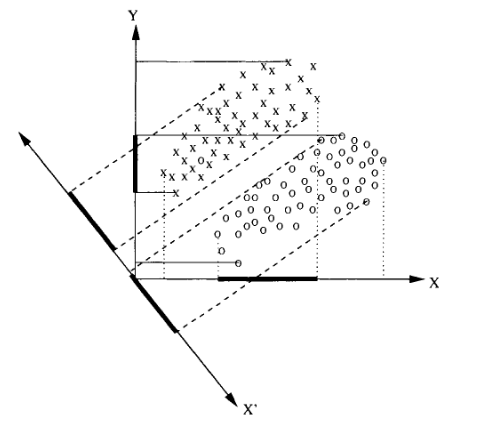
\includegraphics[scale=0.5]{img/explicaciones/dim_reduct.png}
        \end{center}
        \caption{Reducción de dimensionalidad}
        \label{wwww}
    \end{figure}

    En la Figura \ref{wwww}, se representan muestras pertenecientes a dos clases de patrones distintas (denotadas por los simbolos X y O), cuyas coordenadas están representadas por los componentes $X$ y $Y$. Podemos observar que la proyección de las muestras sobre los ejes $X$ e $Y$ se superponen. Por lo tanto,los componentes $X$ y $Y$ no resultan buenos para diferenciar las muestras entre sí. Podemos ver que, en este caso, es posible encontrar un conjunto reducido de componentes que resulte mejor para diferenciar las muestras. Efectivamente, la proyección de las muestras sobre la nueva coordenada ($X'$) muestra que estas no se superponen, lo que que resultaría en un mejor criterio para diferenciarlas.
    
    Una técnica dentro de este enfoque es la denominada PCA \emph{Principal component analysis}, (también conocida como \emph{Karhunen-Loéve transform}). El conjunto reducido de componentes en estes caso, está compuesto por los autovalores de la matriz de covarianza de las muestras. En un principio la elección de esta matriz puede resultar poco intuitivo, pero es generalmente el caso, que en reconocimiento de patrones, nuestras muestras presenten un alto grado de correlatividad \cite{img-proc}.
    
    Siendo $r$ la dimensión de nuestras muestras, llamamos $\boldmath{\mu}$ al vector $r$-dimensional del promedio de las muestras y la $r\times r$ matriz de covarianza $M$ se calculan para los datos de entrenamiento. Luego, obtenemos autovectores con sus autovalores asociados, luego, con los los primeros $\alpha$ autovectores (ordenados en módulo del autovalor asociado en forma descendente) y los introducimos en una matriz por columna, la llamamos $V$. Obtenemos la transformación característica de las muestras haciendo el producto
    
    \[X' = V^t \cdot X^t\]
    
    Donde la dimensión de esta matriz es $N\times \alpha$, donde $N$ es la cantidad de muestras\cite{pattern}.

        \subsubsection{Algoritmo de deflación y método de la potencia}
        Para poder obtener los autovalores y autovectores del método de PCA, tuvimos que implementar algoritmos para poder conseguir estos últimos. Utilizamos el algoritmo de deflación, basándonos en que, si una matriz B de $\mathbb{R}^{nxn}$ posee autovalores que cumplen:
        \begin{align*}
            |\lambda_1| > |\lambda_2| > \hdots > |\lambda_n|
        \end{align*}
        Y una base ortonormal de autovectores, entonces se verifica que:
        \begin{align*}
                B - \lambda_1 v_1 v^{t}_{1}
        \end{align*}
        Tiene autovalores 0, $\lambda_2$,\hdots ,$\lambda_n$. Esto implica que, si obtenemos de alguna manera el primer par de autovalor y autovector, entonces podemos construir una nueva matriz con ese calculo que tendrá el resto de autovalores y el que teníamos antes será 0 ahora. Luego, para conseguir este par de autovalor y autovector, podemos utilizar el método de la potencia. 
        
        Este es un algoritmo iterativo que luego de suficientes iteraciones converge al autovector correspondiente al autovalor mas grande. El algoritmo empieza por un vector aleatorio $x_0$ y la matriz B, de la cual se quiere obtener este primer par de autovalor y autovector. En cada paso iterativo, se multiplica a este vector por la matriz, y luego se lo normaliza. Este proceso se repite la cantidad de veces que uno indique, o hasta que lo diga un criterio de corte. Dependiendo de las iteraciones y el criterio de corte, el resultado puede ser mas o menos preciso, y el tiempo puede ser mayor o menos a su vez.
        
        En nuestro caso, agregamos un criterio de corte, el cual se basa en la siguiente propiedad:
        
        \[  \pint{a,b} &= \norm{a}\norm{b}\cos(\theta) \iff \frac{\pint{a,b}}{\norm{a}\norm{b}} &= \cos(\theta)\]
        
        Como que 2 vectores tienen ángulo 0 cuando son linealmente dependientes sabemos que podemos tomar $\cos{\theta}$ = 1. Luego, por la igualdad anterior, si el termino de la izquierda de la igualdad es 1, sabemos que tenemos 2 vectores linealmente dependientes entre sí. 
        
        Propusimos utilizar esta propiedad para establecer un criterio de corte. Si el calculo de la izquierda aplicado sobre el vector de la iteración anterior y el nuevo es "cercano" a 1, entonces terminamos el algoritmo. Esto implica que es importante encontrar un épsilon tal que, lo que se define como "cercano" no genere un error importante en los autovalores y autovectores asociados. Por estas razones, seleccionamos un épsilon entre un conjunto de posibles opciones, observando como se comportaba cada uno sobre una matriz diagonal que establecimos como parámetro para calcular los errores relativos en los cálculos.
        
        Tomamos como parámetro una matriz cuadrada, con sus filas y columnas de longitud 28*28, para simular el uso real que se le dará, ya que trabajaremos sobre matrices con estas dimensiones. Luego, le aplicamos el método de deflación, que utilizó el método de la potencia, para recuperar los primeros N autovalores. Finalmente evaluamos el promedio del error relativo entre nuestro resultado y el real, y obtuvimos los siguientes resultados:
        
        
        \begin{figure}[H]
            \begin{center}
                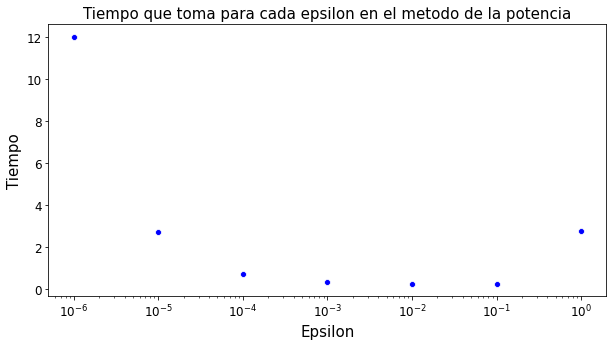
\includegraphics[scale=0.36]{img/explicaciones/eps_time.png}
                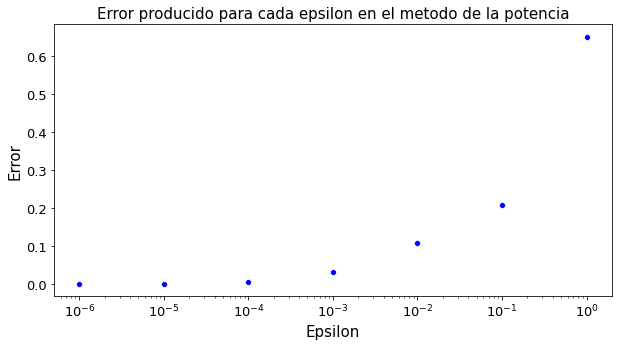
\includegraphics[scale=0.36]{img/explicaciones/eps_error.png}
                \caption{Error producido y tiempo que tomó calcular los primeros 30 autovalores para una matriz diagonal de dimensión 28*28 para distintos valores de épsilon.}
            \end{center}
        \end{figure}
        
        Entonces, vemos que, para un conjunto de épsilon de la forma 10e-i, con i entre 0 y 6, el que mejor se comporta en relación tiempo y error es el épsilon= $10e^{-4}$.
        
     
    \subsection{Parameter Tuning}
    Cuando se trata con clasificadores, estos usualmente involucran parámetros, cuya elección es crucial para lograr un funcionamiento óptimo. Algunos de estos parámetros no son ajustados por el mismo clasificador en la etapa de training, sino que deben ser decididos desde afuera por los que se encuentren diseñando al mismo. Esto implica que, como se mencionó al principio, si se toma una elección pobre de los parámetros, puede terminar en un resultado poco satisfactorio.
    
    Debido a esto, suele haber un gran interés en poder delegarle a alguien mas la tarea de poder encontrar los valores "óptimos" de los parámetros. Como consecuencia, aparece lo que se conoce como \textit{parameter tuning}, que involucra utilizar algoritmos que se encargan de optimizar los parámetros para buscar los mejores posibles. La idea general de su funcionamiento se resume en 2 pasos. Primero se define la función de costo que se quiere minimizar y los parámetros involucrados, y luego el algoritmo explora distintas combinaciones de los parámetros para minimizarla.
    
    Existen múltiples algoritmos que se utilizan para llevar a cabo esta tarea de parameter tunning, pero nosotros optamos por utilizar uno conocido y que suele presentar buenos resultados, llamado simulated annealing.
        
        \subsubsection{Simulated annealing}
        Este algoritmo es uno de los muchos que realizan \textit{parameter tuning}, y busca aproximar al máximo global de la función de costo dada. Es eficiente en encontrar este máximo en espacios discretos, por lo cual decidimos usarlo ya que, nuestros parámetros pueden variar dentro de un rango de valores discreto. 
        
        Este algoritmo esta inspirado en un concepto físico:
        \begin{displayquote}
            ``The name and inspiration come from annealing in metallurgy, a technique involving heating and controlled cooling of a material to increase the size of its crystals and reduce their defects. Both are attributes of the material that depend on its thermodynamic free energy. Heating and cooling the material affects both the temperature and the thermodynamic free energy."
        \end{displayquote}
        
        La idea general de este algoritmo es la de combinar dos conceptos claves a la hora de explorar un espacio para minimizar el costo de una función, \textbf{exploración} y \textbf{explotación}.
        
        \begin{itemize}
            \item \textbf{Exploración}: Buscar en distintos puntos del espacio, sin darle mas importancia a una región, con el objetivo de tener una idea general del costo de la función en distintos puntos del espacio.
            
            \item \textbf{Explotación}: Concentrarse en una región puntual del espacio, con el objetivo de minimizar el costo de la función bajo esa región puntual.
        \end{itemize}
        
        Intenta incorporar estos dos conceptos, para poder beneficiar mas uno que otro dependiendo de la etapa en la que se encuentre. Para decidirlo, considera la \textit{ temperatura del sistema}. Mientras sea alta, se beneficia mas a la exploración, y es mas posible que el algoritmo explore opciones que sean peores de las que ya encontró, con la esperanza de poder encontrar algo mejor mas adelante. Cuando comienza a llegar a niveles bajos, se empieza a beneficiar mas a la explotación, y es menos probable que se acepte temporalmente una peor opción, y mas probable que se intente encontrar el máximo alrededor de la mejor opción que se tenga hasta el momento. 
        
        \begin{figure}[H]
            \begin{center}
                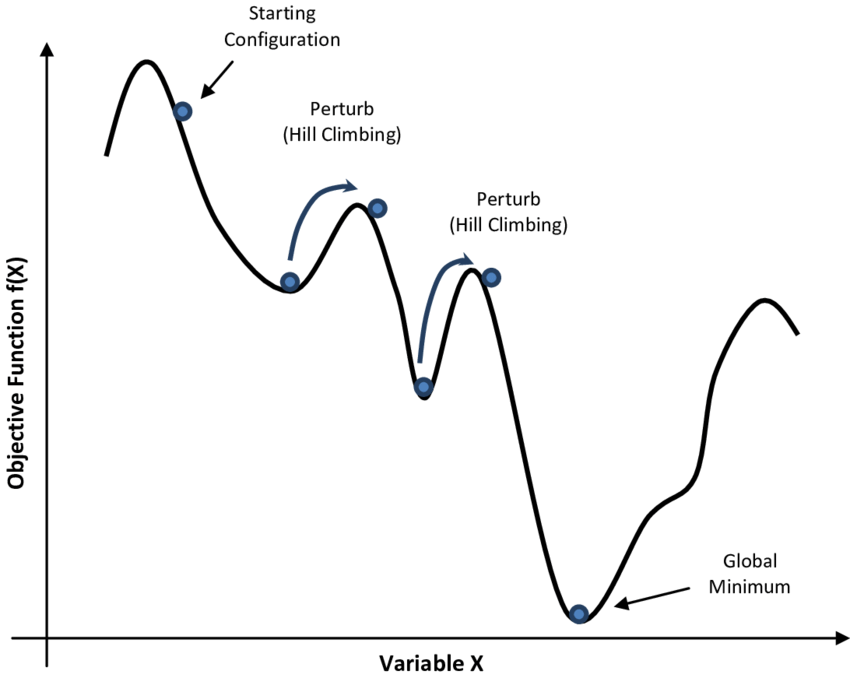
\includegraphics[scale=0.3]{img/explicaciones/Simulated_Annealing.png}
                \caption{Comportamiento de simulated annealing}
                \label{fig:sim-ann}
            \end{center}
        \end{figure}
        
        Con este comportamiento se logra que, al principio el algoritmo pueda salirse de un mínimo local que haya encontrado, y al final pueda concentrarse en mejorar la solución que encontró buscando el mínimo local/global alrededor de ella. Puede observarse en Fig. \ref{fig:sim-ann}
       
        En el uso puntual que se le dará aquí, se definirá la función de costo como:
        \begin{align*}
        f(x) &= 1 - accuracy(x)
        \end{align*}
        Hacemos esto porque a mayor accuracy, menor valor de f(x), con lo cual minimizar esta función es equivalente a maximizar la accuracy. Luego, los parámetros en este caso serán k, si se trata de KNN, o k y $\alpha$ cuando se usa PCA+kNN.

    \subsection{K-Fold cross validation}
    Al aplicar métodos de optimización como los mencionados anteriormente sobre clasificadores, puede optarse por fijar cual va a ser el conjunto de training, y cual el de validation a lo largo del proceso. Luego, se puede aplicar el \textit{parameter tunning} sobre estos dos conjuntos fijos, y obtener los parámetros que optimizan al classifier bajo estos conjuntos de datos. El problema de esto es lo que se mencionó a lo ultimo, se esta optimizando para conjuntos fijos. Esto provoca que al maximizar bajo un mismo conjunto no necesariamente implique que en el caso general sea mejor, ya que no se está optimizando para distintas variaciones de datos.
    
    Una forma de solucionar este problema es la de intentar evaluar bajo distintos conjuntos de training y validation y tomar el promedio de todos ellos. Para esto existe la técnica de K-Fold cross validation, que busca solucionar el problema mencionado aplicando variaciones en los conjuntos para luego evaluar. Podemos ver esto mas claramente en el siguiente diagrama:
    
    \begin{figure}[H]
        \begin{center}
            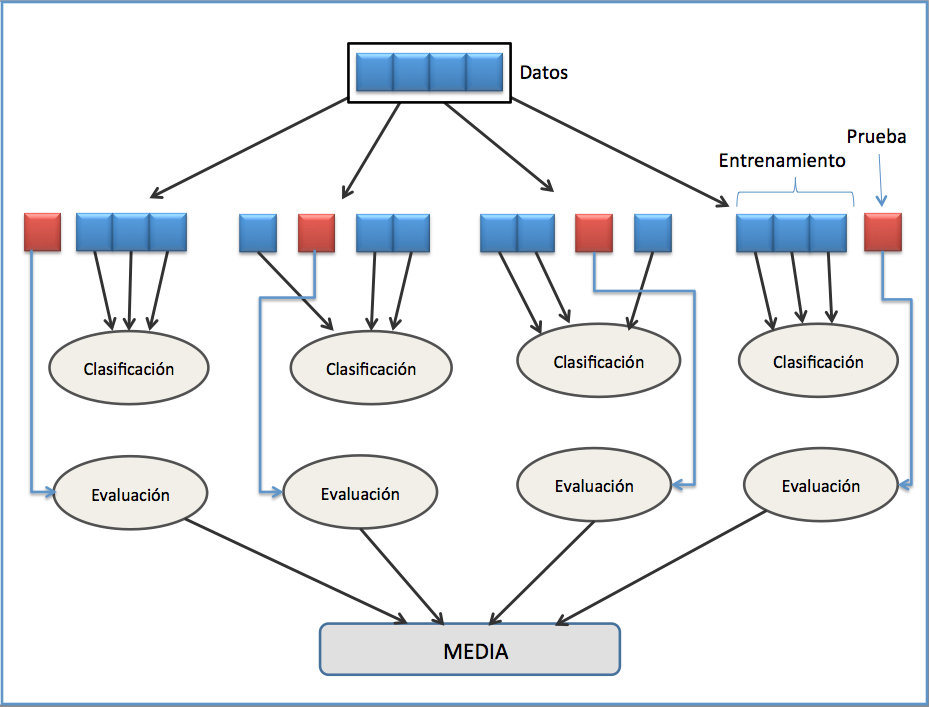
\includegraphics[scale=0.3]{img/explicaciones/k_fold.png}
        \end{center}
    \end{figure}
    
    En este caso particular, se tiene un conjunto de datos que se lo divide en 4 conjuntos de igual tamaño. Luego, se toma en cada caso 3 conjuntos para training (Clasificación) y el otro para validation (Evaluación). Con estos 2 conjuntos de training y de validation, se entrena al modelo y luego se lo evalúa, generando un resultado. Este proceso se repite para cada variación de conjunto de training y validation, y se obtiene la media de los resultados obtenidos. Esta media va a ser entonces el que se va a intentar maximizar bajo el criterio establecido.
        
\section{Experimentación}

    \subsection{Weighted vs normal kNN}\label{exp-knn-weights}
    Como kNN por si solo analiza las imágenes en una dimensión demasiado grande, puede suceder que no estén en \textit{nubes} perfectamente separadas entre sí, y luego que considerar muchos vecinos termine siendo contraproducente, al tomar información de dígitos que no son el deseado, ya que sin importar que tan cerca esté, si es de los más cercanos su voto vale lo mismo. Esto causa que agregar más vecinos solo resulte en más ruido para el clasificador.
    
    Esto nos hizo chocarnos contra la pared al intentar optimizar kNN por si solo. Los $k$ mas chicos tendían a ser los que performaban mejor en cuanto a accuracy. Más aún, siempre daba $k=1$, hasta que llegamos a llamarlo \textit{the curse of $k=1$} (un poor mans \textit{curse of dimensionality}) Para lidiar con esto, proponemos una variación de kNN, en la que el voto de cada vecino no vale por igual.
    
    En particular, tomamos un peso inversamente proporcional a la distancia. Mientras mas cerca estén, mas vale su voto. Esto debería ayudar a que agregar más vecinos no resulte en simplemente ruido.
    
    Además, consideraremos una sofisticación de estos: aquellos que tomen una potencia de la distancia para hacer que las diferencias sean aún más pronunciadas.

    \subsection{Optimizando kNN}\label{exp-knn-opt}
    Previo a la optimización de kNN, haremos un simple barrido lineal de diferentes $k$ s para tres variaciones de kNN y optimizaremos el ganador: \textbf{uniform} (i.e donde el peso de cada voto es uniforme, equivalente a que no haya weights), \textbf{distance} donde se toma como weight $1/distance$ y finalmente \textbf{distance\_pow}, que toma $1/(distance)^3$ lo cual hace que las diferencias sean mas pronunciadas.
    
    Nuestra hipótesis es que el mejor será el último, al ser mas sofisticado que los demás.
    
    Para optimizarlo, intuimos que si bien el $k$ resultante será bajo, debería ser mayor a uno, ya que siempre brinda más información agregar algunos vecinos cuando sus votos no pesan lo mismo.
    
    \subsection{Optimizando kNN+PCA}\label{exp-knn+pca-opt}
    Las posibles combinaciones de k y alpha que existen son muchas, lo cual implica que no es razonable intentar cada una para determinar cual es la mejor. Por estos motivos, decidimos utilizar el algoritmo de optimización Simulated Annealing para poder evaluar menos combinaciones e intentar llegar al mismo resultado que resultaría en probar todas las combinaciones existentes. A su vez, los rangos de K y $\alpha$ se encuentran acotados por la cantidad de imágenes y el tamaño de las mismas respectivamente, pero nosotros tomamos un rango aun mas acotado para explorar.
    
    También, como se mencionó en un punto previo, llevamos a cabo dos optimizaciones distintas, variando el criterio de selección de kNN entre Weighted y Uniform. Por un lado vemos como se comporta la versión de kNN donde la votación se lleva a cabo de manera uniforme, sin tener en cuenta las distancias de los K vecinos mas cercanos, y nos concentramos en optimizarlo en conjunto con PCA. Por el otro lado, repetimos el mismo proceso pero cambiando el criterio de votación, utilizando el Weighted, para ver como afecta que cada voto tenga un peso basado en su distancia.
    
    En ambos casos seguimos el mismo procedimiento, definimos el siguiente rango para los parámetros (K,$\alpha$):
    \begin{align*}
    0 \leq    K   \leq  100\\
    0 \leq   \alpha   \leq  100
    \end{align*}
    En conjunto con la función de costo, que consiste del método de K-Fold sobre el conjunto de imágenes, y aplicando en cada fold la función de accuracy mencionada previamente. Luego, utilizando este rango para el algoritmo de Simulated Annealing, obtuvimos la combinación óptima ,o al menos cercana a ella, de (K,$\alpha$) para el rango definido. Además de esto, aprovechando el algoritmo de Simulated Annealing, guardamos las combinaciones que se exploraron en cada iteración del mismo, para luego poder ver la evolución a lo largo de cada paso. Con esto buscamos ver como se comporta la función de accuracy aplicada sobre el espacio de (K,$\alpha$), para poder entender mejor como se relacionan estas variables entre sí.
    
    Dicho todo esto, suponemos que al combinar kNN con PCA, el K de kNN resulta mas grande que en kNN sin ningún extra, ya que al incluir PCA las imágenes transformas pasan a tener menos redundancia entre ellas, haciéndolo mas efectivo el incluir más para clasificar. A su vez, el nuevo parámetro $\alpha$ creemos que debe ser mayor K, entre valores alrededor de 30 y 50, aunque esto depende también de los datos de training que se usen. Esto ultimo lo decimos porque sabemos que, cada nuevo valor $\alpha_i$ aporta nueva información, pero siempre menor que el anterior, lo que implica que al incluir un numero suficiente se obtiene algo cercano al $100\%$ de las características importantes con los mismos. Esto creemos que provoca que, no sea beneficioso a partir de cierto punto incluir más, y por esto mismo decimos que la cota se encuentra en el rango mencionado.

    \subsection{Influencia del tamaño de la muestra y K de K-fold}\label{exp-sample-size}
    Si bien estamos optimizando los parámetros de los clasificadores, para cada experimento debemos elegir ciertos \textit{metaparametros}, de las herramientas que utilizamos para evaluarlos. Entre ellos, están el tamaño de la muestra que tomamos para entrenar y testear, y la cantidad de folds a realizar.
    
    En cuanto al tamaño de la muestra, suponiendo que se hace un sample uniforme de la muestra original, creemos que mientras mas chica sea peor va a ser la performance. Esto es porque al entrenar con menos datos, el clasificador cuenta con menos información, y por lo tanto peores son sus predicciones. Por ejemplo, viéndolo desde el punto de vista de kNN, mientras menos datos tenemos menos vecinos útiles tendrá cada píxel.
    
    Sobre K-Fold, mientras mas grande sea el K, proporcionalmente se entrena sobre más y se testea sobre menos, que es lo opuesto a reducir el tamaño de la muestra. Esto debería desembocar en mejores resultados, ya que hay menos que predecir y mucha más información.
    
    \subsection{Kappa de Cohen}
    
    Además de obtener los valores óptimos para los parámetros involucrados en cada classifier propuesto, nos interesó ver que estaba pasando dentro de la clasificación del mismo. Nos preguntamos como se comportaba con cada clase de dígito, si estaba fallando en el dígito 8 por ejemplo, porque faltaba ser más optimizado. O por el otro lado, si se trataba de una clase de dígito que resultaba compleja de clasificar en general por cualquier clasificador.
    
    Para abordar esta pregunta entonces, decidimos incorporar a nuestro análisis otro clasificador, con el objetivo de poder comparar ambos clasificadores, y por lo tanto poder contestar estas preguntas que planteamos previamente. Como el objetivo era compararlos, decidimos utilizar la métrica llamada Kappa de Cohen, la cual busca analizar el nivel de concordancia entre dos clasificadores al momento de clasificar un conjunto de datos. 
    
    Al obtener el nivel de concordancia, en conjunto con la accuracy de ambos clasificadores, se puede determinar sí una clase de dígito es difícil para un clasificador en particular, o es un problema para ambos. Con esto buscamos poder determinar que clase de dígitos presenta un desafió a los clasificadores en general, mas allá de la capacidad de clasificar del mismo. Dicho esto, pensamos que las clases que parecen presentar mayor conflicto son la del 8 y el 3, ya que estos dígitos tienden a verse muy similares, al igual que el 6 y el 5.

    \subsection{Tiempos de ejecución}
    Al tener ambos clasificadores optimizados, al margen de cuál es mejor en cuanto a accuracy u otras métricas, hay que tenér en cuenta el tiempo de ejecución. Aunque kNN+PCA fuera peor, tendría muy a favor que debería ser muchísimo más rápido, ya que al reducir la dimensionalidad con PCA kNN correría más rápido. Y kNN de por sí debería ser más lento en todos los casos, ya que itera la imagen de train por cada fila de la imagen de predict para ver las distancias.

\section{Resultados y discusión}

    \subsection{El mejor tipo de kNN}
    Para ver cual kNN era el mejor, decidimos hacer un pequeño barrido lineal sobre una selección de $k$s y ver como daba el accuracy para cada weight.
    
    \begin{figure}[H]
        \begin{center}
            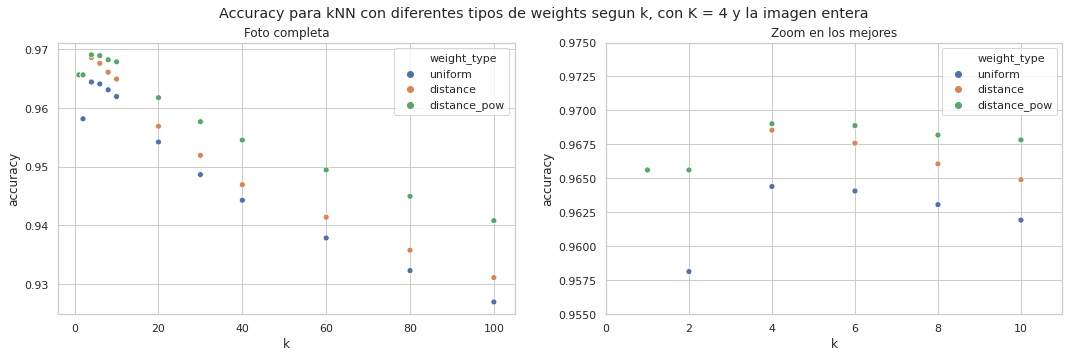
\includegraphics[scale=0.425]{img/exp/knn/knn_weights.png}
            \caption{Accuracy para kNN variando el tipo de weight}
            \label{exp-knn-weights}
        \end{center}
    \end{figure}
    
    Como se puede ver en la Figura \ref{exp-knn-weights}, mientras mas chico es el k, es estrictamente mejor el accuracy resultante. Sin embargo, el hecho de tomar pesos para los votos hace que el impacto sea mucho menor, como habíamos intuido. Además, tomar la distancia cúbica es estrictamente mejor para casi todos los casos, pero de todas formas el accuracy decrece, por lo que agregar vecinos sigue sumando ruido, solamente menos. El mejor k observado aqui, aunque no fue producto de ninguna optimización interesante, es 4.
    
    \subsection{Optimización de kNN}
    A la hora de optimizar kNN, optamos por lo mismo que el resto: el algoritmo de \textit{Simulated Annealing}.
    
    \begin{figure}[H]
        \begin{center}
            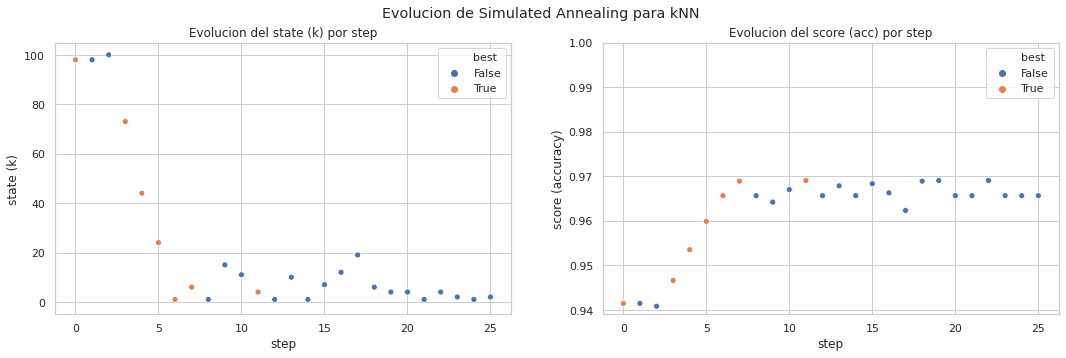
\includegraphics[scale=0.425]{img/exp/knn/knn_sim_ann_evol.png}
            \caption{Evolución de Simulated Annealing para kNN con weights cúbicos. En naranja los que el algoritmo consideró mejores}
            \label{exp-knn-sim-ann-evol}
        \end{center}
    \end{figure}
    
    En la Figura \ref{exp-knn-sim-ann-evol} se puede apreciar la evolución del algoritmo en cada paso. Luego de comenzar de forma aleatoria en un valor cercano al 100, rápidamente comienza a bajar en picada encontrando valores mejores uno atrás del otro, hasta que en un momento llega al mejor, luego del cual no encuentra otro. Como sospechabamos, a menor k, mejor score.
    
    \begin{figure}[H]
        \begin{center}
            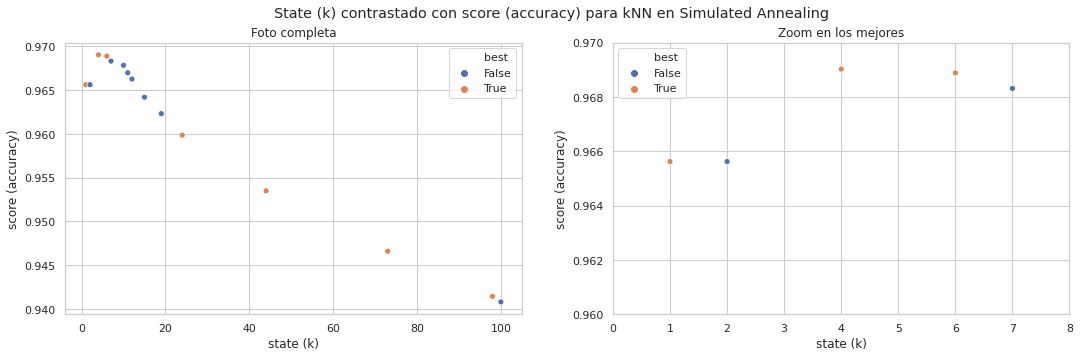
\includegraphics[scale=0.425]{img/exp/knn/knn_sim_ann.png}
            \caption{Accuracy para kNN variando el tipo de weight}
            \label{exp-knn-sim-ann}
        \end{center}
    \end{figure}
    
    En la Figura \ref{exp-knn-sim-ann} se puede ver la relación entre k y el accuracy, similar a en Fig. \ref{exp-knn-weights}, con los weights. Haciendo zoom, podemos ver que el mejor coincide con el encontrado previamente con el barrido lineal, $k = 4$, con $k=6$ pisándole los talones. Se pueden ver los numeros exactos en la Figura \ref{knn-optimization-results}

    \begin{figure}[H]
        \begin{center}
        \begin{tabular}{ |c|c| } 
        \hline
        \textbf{State (k)} & \textbf{Score (accuracy)} \\
        \hline
        4 &     0.9690 \\
        6 &     0.9688 \\
        7 &     0.9683 \\
        10 &    0.9678 \\
        11 &    0.9669 \\
        12 &    0.9662 \\
        2 &     0.9656 \\
        1 &     0.9656 \\
        15 &    0.9641 \\
        19 &    0.9623 \\
        24 &    0.9598 \\
        44 &    0.9535 \\
        73 &    0.9465 \\
        98 &    0.9414 \\
        100 &   0.9408 \\
        \hline
        \end{tabular}
        \end{center}
        \caption{Resultados de la optimización de kNN}
        \label{knn-optimization-results}
    \end{figure}
    
    \subsection{Optimización de kNN+PCA}
      A continuacion se muestra la optimizacion para los dos modelos de kNN+PCA, uniforme y weighted, utilizando Simulated Annealing para k y $\alpha$ dentro del rango indicado en la descripción de este experimento.
      
      \subsubsection{Uniforme}
    \begin{figure}[H]
            \centering
            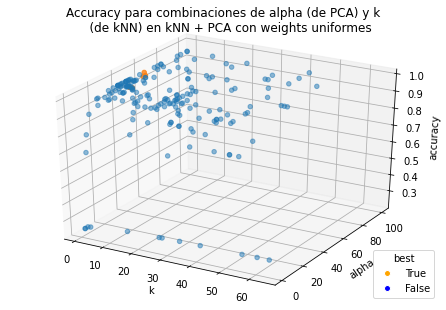
\includegraphics[scale=0.5]{img/exp/pca/opt_knn_pca_unif.png}
            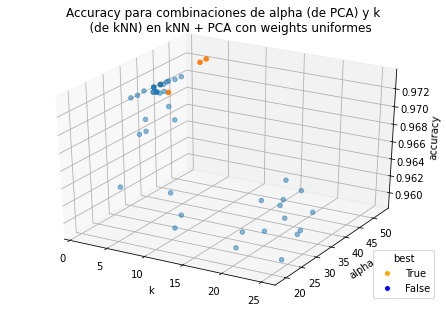
\includegraphics[scale=0.5]{img/exp/pca/opt_knn_pca_unif_zoomed.png}
            \caption{Optimización de kNN+PCA con votación uniforme para kNN, con el gráfico de la derecha siendo un ``zoom" de una parte del de la izquierda. Los puntos naranjas son la evolución de la mejor solución que fue encontrando la optimización en distintas iteraciones.}
            \label{fig:knn-pca-unif}
    \end{figure}
      En la Figura \ref{fig:knn-pca-unif} se puede observar como fue la evolución de Simulated Annealing, a través de todos los estados que fue recorriendo en cada iteración del mismo. Podemos ver en el gráfico de la izquierda como la nube de buenas soluciones siempre involucraba un $\alpha$ mas grande que 5-10, lo cual es razonable porque a pocos valores de $\alpha$, se tiene poca información de las características del problema. 
      
      Además, los valores de K que fueron mas útiles se encontraban en los valores bajo, alrededor del 20 para abajo, lo cual es interesante porque, es razonable pensar que al tener menos redundancia entre los puntos es mejor considerar más, pero no es tal el caso.
      
      Finalmente, podemos ver en el gráfico derecho, que presenta un zoom sobre las mejores soluciones, que pareciera ser que las combinaciones óptimas de valores de parámetros se encuentra en el intervalo de 1 a 10 para K, y de 30 a 50 para $\alpha$. Esto verifica lo que supusimos sobre el valor de $\alpha$, pero difiera con nuestra suposición sobre el valor de K, que pensabamos que iba a ser mas alto que lo que terminó siendo.
    \subsubsection{Weighted}
    A continuación mostramos los resultados de la búsqueda de los mejores parámetros de $\alpha$ y $\kappa$, para el clasificador \emph{kNN} entrenado con muestras transformadas por \emph{PCA}.
    
    \begin{figure}[H]
            \centering
            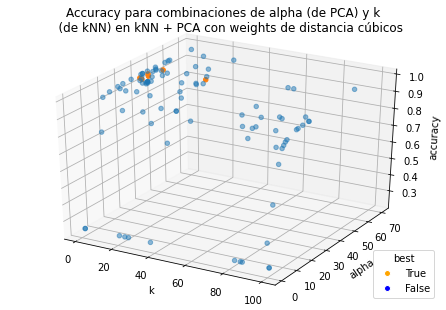
\includegraphics[scale=0.5]{img/exp/pca/opt_knn_pca_weight.png}
            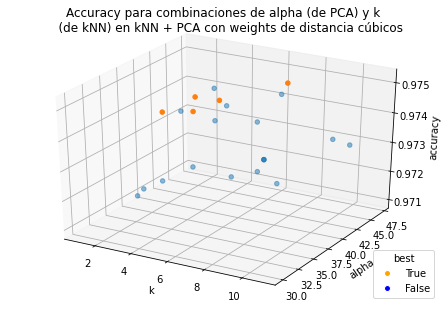
\includegraphics[scale=0.5]{img/exp/pca/opt_knn_pca_weight_zoomed.png}
            \caption{Optimización de kNN+PCA con votación weighted para kNN}
            \label{fig:knn-pca-weight}
    \end{figure}
    
    Se puede observar como, al cabo de $100$ iteraciones, los mejores resultados (mostrados en naranja), se fueron acomodando cerca a $6, 33$ para $\kappa$ y $\alpha$, respectivamente. 
    Para estos resultados, la métrica de \emph{accuracy} del clasificador estuvo cercana al elusivo $98\%$ (Figura \ref{fig:knn+pca-optimization-results}).
    
    Se puede ver que, los parámetros optimizados por el algoritmo de \emph{simmulated annealing} no varían de manera significativa al utilizar un clasificador \emph{kNN} cuyos votos estén ponderados de manera uniforme versus un clasificador \emph{kNN} cuyos votos estén ponderados basados en sus distancias a la muestra a evaluar. Lo que si mostró una diferencia significativa fueron resultados de métricas como la antes mencionada \emph{accuracy}. Estos resultados se pueden ver más en detalle en la Figura \ref{fig:knn+pca-optimization-results}.
    
    
    \begin{figure}[H]
        \centering
        \begin{tabular}{ |c|c| } 
        \hline
        \textbf{state} (k, $\alpha$)  & \textbf{accuracy}   \\
        \hline
        (6, 33)&  0.975 \\
        (6, 37)&  0.975 \\
        (8, 37)&  0.974 \\
        (7, 45)&  0.974 \\
        (7, 44)&  0.974 \\
        (5, 34)&  0.974 \\
        (4, 42)&  0.974 \\
        (4, 39)&  0.974 \\
        (4, 34)&  0.974 \\
        (11, 40)& 0.974 \\
        (11, 33)& 0.974 \\
        (10, 32)& 0.974 \\
        (10, 32)& 0.974 \\
        (10, 32)& 0.974 \\
        \hline
        \end{tabular}
        \quad
        \begin{tabular}{ |c|c| } 
        \hline
        \textbf{state} (k, $\alpha$)  & \textbf{accuracy}   \\
        \hline
        (5, 34) & 0.973 \\
        (5, 34) & 0.973 \\
        (6, 34) & 0.972 \\
        (6, 34) & 0.972 \\
        (5, 35) & 0.972 \\
        (4, 34) & 0.972 \\
        (4, 34) & 0.972 \\
        (3, 53) & 0.972 \\
        (3, 51) & 0.972 \\
        (4, 36) & 0.971 \\
        (3, 64) & 0.971 \\
        (3, 45) & 0.971 \\
        (3, 44) & 0.971 \\
        (3, 43) & 0.971 \\
        \hline
        \end{tabular}
        \caption{Resultados para kNN+PCA con weights de distancia (izq) y uniforme (der) }
        \label{fig:knn+pca-optimization-results}
    \end{figure}
    
    \subsection{Influencia de K y el tamaño de la muestra}
    Para este experimento, variamos todas las posibilidades para dos conjuntos de K (de K-Fold) y \textit{sample size}, para determinar cuanto de la muestra de imagenes tomamos para el train y test.
    \subsubsection{kNN}
    Como se puede ver en la Figura \ref{fig:knn-variaciones-acc}, el clasificador kNN se comporta como era esperado, ya que a mayor tamaño de imagen y mayor K de K-fold el accuracy es mayor.
    
    \begin{figure}[H]
        \centering
        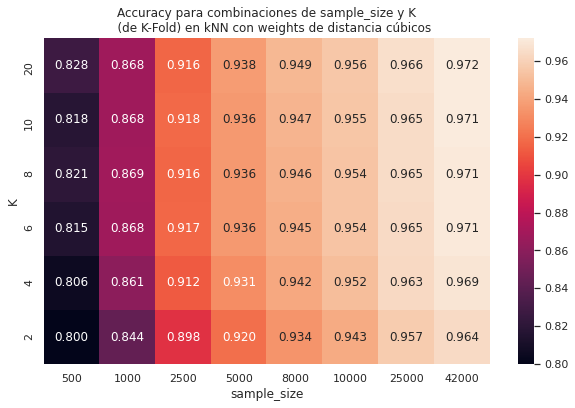
\includegraphics[scale=0.65]{img/exp/knn/knn_variaciones.png}
        \caption{Accuracy para combinaciones de K y tamaño de imagen}
        \label{fig:knn-variaciones-acc}
    \end{figure}
    
    Curiosamente, la Figura \ref{fig:knn-variaciones-f1} muestra que para la métrica F1, nuestra hipótesis no siempre es cierta, ya que para imágenes mas chicas aumentar el K la empeora. No supimos encontrar una razón para este comportamiento.
    
    \begin{figure}[H]
        \centering
        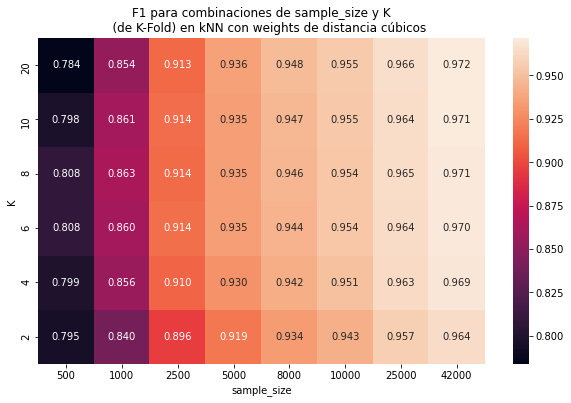
\includegraphics[scale=0.65]{img/exp/knn/knn_variaciones_f1.png}
        \caption{F1 para combinaciones de K y tamaño de imagen}
        \label{fig:knn-variaciones-f1}
    \end{figure}

   
    \subsubsection{kNN+PCA}
    Como podemos ver en la Figura \ref{fig:vars-knn-pca}, ambos clasificadores se comportaron de la misma manera, y a su vez igual que kNN. Pero aquí es mucho mas evidente la mejoría de accuracy al aumentar el K, ya que se pasa a casi 0.98 de 0.971.

    \begin{figure}[H]
            \centering
            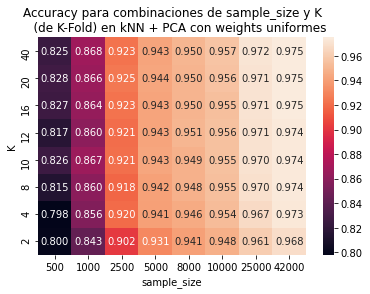
\includegraphics[scale=0.5]{img/exp/pca/vars_knn_pca_unif.png}
            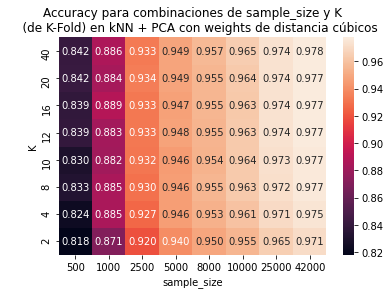
\includegraphics[scale=0.5]{img/exp/pca/vars_knn_pca_weight.png}
            \caption{Variaciones de K y sample size para kNN+PCA uniforme y weighted}
            \label{fig:vars-knn-pca}
    \end{figure}

    \subsection{Kappa de Cohen}
    En la Figura \ref{tab:kappa} a continuacion podemos ver para cada digito, la accuracy de los dos classifiers usados, kNN y kNN + PCA, asi también como la concordancia indicada por la Kappa de Cohen.
    
    \begin{figure}[H]
    \centering
    \pgfplotstabletypeset[
        col sep=comma,
        precision=3,
        columns/0/.style={column name=Digit, column type={|c}},
        columns/accuracy_knn/.style={column name= kNN accuracy, column type={|c}},
        columns/accuracy_knn_pca/.style={column name= kNN + PCA accuracy, column type={|c|}},
        columns/kappa/.style={column name= Cohen's Kappa score, column type={|c|}},
        every head row/.style={before row=\hline,after row=\hline},
        every last row/.style={after row=\hline},
        ]{csv/kappa.csv}
    \caption{Resultados de Kappa de Cohen para kNN comparado con kNN+PCA}
    \label{tab:kappa}
    \end{figure}

    Por un lado, vale notar que hay dígitos que presentan una accuracy cercana al 100\% en ambos classifiers, como en el caso del 0, 1 y 6. A su vez, para estos últimos dígitos el score de Cohen indica aproximadamente un 70\% de concordancia, esto nos dice que ambos classifiers difieran en un 30\% para coincidir en estos tres dígitos, lo cual muestra que existe espacio para mejoras en ellos. 
    
    También vale notar que, el score mas bajo se corresponde al 8, seguido por el 9, lo cual coincide parcialmente con lo que pensamos sobre que el 8 iba a ser complejo para clasificar. Sin embargo, el score de Cohen es alrededor del 60\%, lo cual indica que no parece ser un problema general para el conjunto de estos dos clasificadores, ya que cada uno esta clasificando correctamente un conjunto de 8s que el otro no. Esto nos dice que lo que pensamos en un principio, al menos utilizando estos dos clasificadores para el razonamiento,  no era tan correcto. 
    
    Pensamos que el problema que tuvo este experimento fue que, solo hicimos el análisis considerando nuestros dos clasificadores, que se basan en el mismo principio de kNN. Esto genera resultados que no reflejan la realidad, porque un análisis real debería haber considerado muchos mas clasificadores para tener una muestra mas grande y mayor variedad.
%\begin{figure}[H]
%    \begin{subfigure}{.5\textwidth}
%        \centering
%        \includegraphics[scale=0.275]{graphs/threadsCarga.jpeg}
%        \caption{Rendimiento según cantidad de threads en la carga de %archivos (en $ms$)}
%        \label{res-carga}
%    \end{subfigure}
%    \begin{subfigure}{.5\textwidth}
%        \centering
%        \includegraphics[scale=0.275]{graphs/threadsMaximo.jpeg}
%        \caption{Rendimiento según cantidad de threads en la búsqueda del %máximo (en $\mu s$)}
%        \label{res-max}
%    \end{subfigure}
%\end{figure}

    \subsection{Tiempos de ejecución}
    Para este experimento, iteramos varias corridas normales (sin hacer cross validation, ni ver que tan bueno fue el resultado) de cada clasificador varias veces y tomamos \textit{splits} diferentes para hacer train y test del set de datos, ya que hacer siempre el mismo, por ejemplo 80\% para train y 20\% para test, favorecería al clasificador que tenga el train más veloz.
    
    \begin{figure}[H]
            \centering
            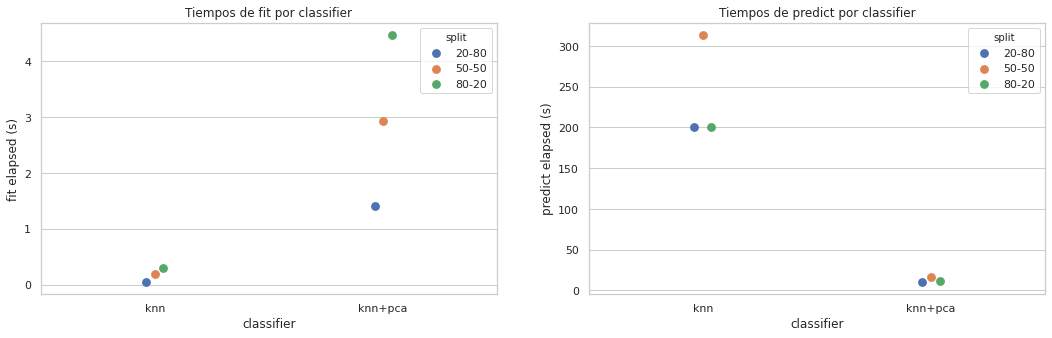
\includegraphics[scale=0.425]{img/exp/time/time_by_stage.png}
            \caption{Tiempos de ejecucion de cada etapa}
            \label{fig:time-step}
    \end{figure}
    
    Como se puede ver en Fig. \ref{fig:time-step}, claramente predict es lo mas caro para kNN y fit para kNN+PCA. Una observación interesante también es que predict tiene los mismos tiempos de ejecución para splits simétricos en kNN, lo cual es razonable ya que su complejidad a alto nivel se puede expresar como O(n * m) donde n es el tamaño de train y m de test. Luego swapearlos no tiene ningún efecto.
    
    Sin embargo, con este gráfico nos resulta difícil ver de forma clara quien es más rápido.
    
    \begin{figure}[H]
            \centering
            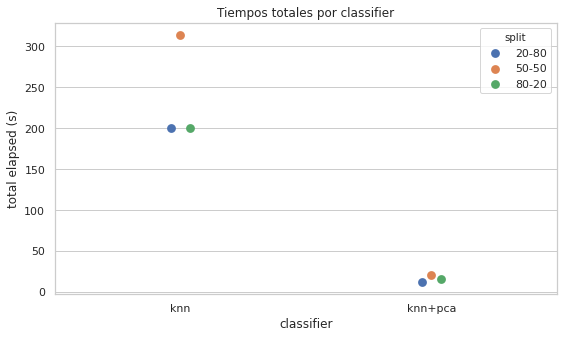
\includegraphics[scale=0.6]{img/exp/time/time.png}
            \caption{Tiempos de ejecución totales (i.e fit + predict)}
            \label{fig:time-total}
    \end{figure}
    
    En Fig. \ref{fig:time-total} se puede ver claramente que para todos los splits, kNN es mas lento que kNN+PCA, lo cual concuerda con lo que suponíamos que iba a suceder. 

\section{Conclusión}

Luego de haber realizado las experimentaciones para las variaciones, y optimizar kNN y kNN con PCA por separado, concluimos que el mejor clasificador es kNN con $k=6$ y votos pesados según la distancia cúbica, junto con PCA $\alpha=34$. Y no solamente en cuanto a \emph{accuracy}, sino también ampliamente en tiempos de ejecución. Así mismo, vimos que aumentando la cantidad de \emph{folds} con los cuales se hace \emph{cross validation}, al igual que la cantidad de imágenes de entrenamiento, en todos los casos, los resultados de la métrica de \emph{accuracy}, mejoran. También pudimos determinar que, hay ciertas clases dentro de los dígitos a reconocer que presentan mejoras en cuanto a su reconocimiento cuando es utilizado el classificador de kNN con PCA, no obstante, todavía hay lugar para optimizar. Con todo esto decidido, pasamos a subirlo a la competencia \textit{Digit Recognizer}\footnote{https://www.kaggle.com/c/digit-recognizer/submissions} de kaggle, y en la figura \ref{fig:kaggle} se pueden ver los resultados, 0.97485, lo cual coincide con nuestra experimentación sobre el conjunto de datos etiquetado.

\begin{figure}[H]
    \centering
    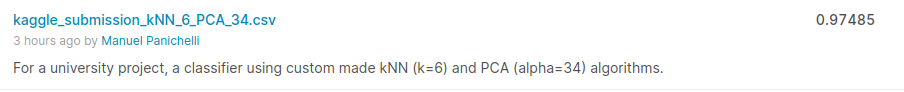
\includegraphics[scale=0.5]{img/kaggle.png}
    \caption{Resultado del \textit{submission} a Kaggle}
    \label{fig:kaggle}
\end{figure}


\begin{thebibliography}{9}

\bibitem{img-proc} 
Tinku Acharya and Ajoy K. Ray. 
\textit{Image Processing Principles and Applications}. 
John Wiley & Sons, 2005.

\bibitem{pattern} 
Richard O. Duda, Peter E. Hart and David G. Stork.
\textit{Pattern classification}.
John Wiley & Sons, 2001.

\end{thebibliography}

\end{document}
